\section{Styles}
\subsection{Schriftart}
Durch den Common-Component Text können wir jedem Text in der App eine einheitliche Schriftart geben.
Ich entschied mich für die Font Poppins \cite{poppins}.

\subsection{Farbwerte}
Alle Farben, die man in der App sehen kann, wurden in der Datei Colors.js in root/styles festgelegt.
So muss nicht, sollte sich das Design ändern müssen, in jedem StyleSheet jede Farbe einzeln
getauscht werden.

Die Hauptfarbe der App ist der wunderschöne Grünton Jade (\#00A86B), welchen ich durch die Webseite
color-name.com \cite{colorName} fand. Die Webseite MyColor.Space \cite{myColorSpace} erzeugt anhand
einer Farbe mehrere andere Farben, die gut dazu passen.

\subsection{Icons}
Die Bibliothek react-native-vector-icons \cite{reactNativeVectorIcons} war eine große Hilfe bei der
Erstellung des Designs. Icons sind nämlich der perfekte Weg, um Informationen in wenig Platz
darzustellen, z.B. welche Funktion ein Knopf hat. Ich habe stets darauf geachtet diverse Icons von
verschiedenen Anbietern in die App einzubauen. Hauptsächlich verwendete ich die
MaterialCommunityIcons, eine große Sammlung von Icons orientiert am Material Design, einer
Designsprache entwickelt von Google.

\subsection{FlashMessage}
\begin{lstlisting}
const App = () => (
    ...
    <FlashMessage position="top" />
    ...
);

export default App;
\end{lstlisting}

Die Komponente FlashMessage ist für Mitteilungen über Geschehnisse in der App zuständig, z.B.
Login fehlgeschlagen oder Login erfolgreich.

\begin{figure}[H]
  \centering
  \hfill
  \subfigure[Login-Informationen falsch]{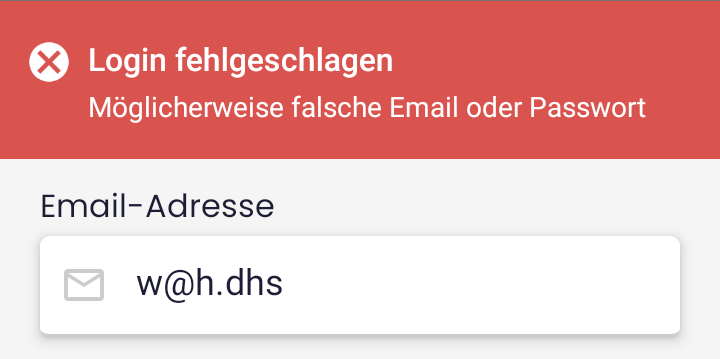
\includegraphics[width=0.4\textwidth]{Mobile/Auth/failed.png}}
  \hfill
  \subfigure[Login-Informationen richtig]{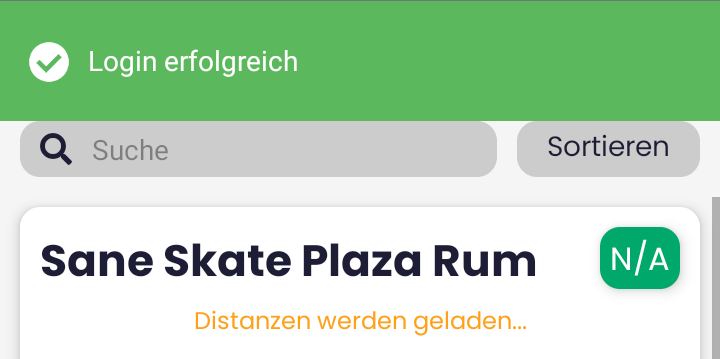
\includegraphics[width=0.4\textwidth]{Mobile/Auth/granted.png}}
  \hfill
  \caption{FlashMessage Beispiel}
\end{figure}